\chapter{Green-Kubo theory of heat transport}  \label{ch:green-kubo}

Our microscopic understanding of heat and mass transport in extended systems is rooted in the Green-Kubo (GK) theory of linear response \cite{Green1954,Kubo1957a}, as applied to the Navier-Stokes equations for the densities of the conserved extensive variables \cite{Kadanoff1963,Forster1975}, which include energy, momentum, and the particle numbers for each molecular species. 
\begin{LEtext}

This work was initiated by Onsager in the thirties \cite{Onsager1931a,Onsager1931b} and carried on by Green and Kubo in the fifties with the theory of linear response \cite{Green1952,Green1954,Kubo1957a,Kubo1957b}. The theory is built on the concept of adiabatic decoupling of the slow long-wavelength components of the densities of conserved extensive quantities (which include energy, momentum, and particle number) \cite{Kadanoff1963}, the so-called \emph{hydrodynamic variables}, from the other atomically fast degrees of freedom. Their work resulted in the celebrated \emph{Green-Kubo equations}, a consequence of the fluctuation-dissipation theorem, that establish a relation between a (non-equilibrium) transport coefficient $\kappa$ and the spontaneous fluctuations of the relevant currents $J$ at equilibrium. Transport coefficients are in fact proportional their autocorrelation times:
\begin{equation}
\kappa\propto\int_{0}^{\infty}\!\langle{J}(t){J}(0)\rangle\, dt, \label{eq:GK}
\end{equation}
where the brackets indicate ensemble averages over trajectories, and are accessible to equilibrium MD simulations.

In this chapter we briefly walk through the theory that allows the derivation of the Green-Kubo equations for transport coefficients, starting from the definition of the hydrodynamic variables of a system, and the use of the linear response theory to connect equilibrium properties to non-equilibrium ones. We then specialize to the case of heat transport in solids and one component fluids, and the particular case of multi-component fluids, and we derive the expression of the energy flux for systems described by classical force fields.
\end{LEtext}


\section{Hydrodynamic variables} \label{sec:hydrodyn_var}
The macroscopic processes occurring in condensed matter are often described in terms of \emph{extensive variables}. By definition, the value that such a variable assumes for a system is the sum of the values it has for each of its subsystems. This property allows one to express an extensive variable, $A$, as the integral of a suitably defined density, $a(\mathbf{r})$, as:
\begin{equation}
A[\rOmega]=\int_\rOmega a(\mathbf{r})d\mathbf{r}, \label{eq:A-extensivity}
\end{equation}
where $\rOmega$ is the system volume. Here and in the following boldfaces indicate 3D vectors and Greek subscripts label Cartesian components: $\mathbf{u}= \{u_\alpha\} = \{u_1,u_2,u_3\}$. When an extensive quantity is locally conserved, a current density, $\bm{j}(\mathbf{r},t)$, can be associated to its density in such a way that the two of them satisfy the continuity equation:
\begin{equation}
\frac{\partial a(\mathbf{r},t)}{\partial t} = - \nabla\cdot\bm{j}(\mathbf{r},t), \label{eq:continuity}
\end{equation}
where $\nabla\cdot\bm{j}$ indicates partial differentiation and the middle dot a scalar product (a divergence in this case). In the following the densities and current densities of conserved quantities will be called \emph{conserved densities} and \emph{conserved currents} for short. The space Fourier transform of Eq.~\eqref{eq:continuity} reads:
\begin{equation}
\dot{\tilde a}(\mathbf{q},t) = - i\mathbf{q} \cdot \tilde {\bm{\jmath}} (\mathbf{q},t), \label{eq:kontinuity}\end{equation}
where the overdot indicates a time derivative and the tilde a Fourier transform, so that the longer the wavelength, the slower is the dynamics of a conserved density. We conclude that for long enough wavelengths, conserved densities are adiabatically decoupled from all the other (zillions of) fast atomic degrees of freedom. Note that in this chapter we are using the concept of \emph{adiabatic decoupling} in two distinct senses, depending on the context: to indicate the decoupling of electronic from nuclear degrees of freedom, and that of hydrodynamic variables from fast atomic ones.

The long-wavelength Fourier components of conserved densities are called \emph{hydrodynamic variables}. In macroscopically homogeneous systems, different wavelengths are decoupled from each other, while, as we have seen, the long wavelengths are adiabatically decoupled from all the other degrees of freedom. Let us suppose there are $Q$ conserved extensive variables. In the case of a mono-atomic fluid, for instance, $Q=5$, corresponding to mass (or particle number), energy, and the three components of the momentum. In order to simplify the notation, we set the value of the conserved quantities equal to zero, $A^i=0$, so that their densities, $a^i(\mathbf{r})$, directly refer to the departure from equilibrium, and we indicate by $\bm j^i(\mathbf{r},t)$ the corresponding currents. At equilibrium, all the conserved densities and currents vanish. Off equilibrium, it will be assumed that the wavelength and the time scale of the disturbances are so long that thermal equilibrium still holds \emph{locally}. That is to say, a local temperature, pressure, and chemical potential can be defined, such that, when combined with the densities of extensive variable, they satisfy a local equation of state.

For small enough deviations from equilibrium, the time derivatives of conserved densities are linear combinations of the densities themselves. In the frequency/wavevector domains this condition can be expressed as
\begin{equation}
  -i\omega\tilde a^i(\mathbf{q},\omega) = \sum_j \tilde\rLambda^{ij}(\mathbf{q},\omega) \tilde a^j(\mathbf{q},\omega), \label{eq:Fourier-continuity}
\end{equation}
where the tilde indicates now a space-time Fourier transform: $\tilde a(\mathbf{q},\omega) = \int \mathrm{e}^{-i(\mathbf{q}\cdot \mathbf{r}-\omega t)} a(\mathbf{r},t)d\mathbf{r}dt $. By combining Eq.~\eqref{eq:Fourier-continuity} with the time Fourier transform of Eq.~\eqref{eq:kontinuity}, we obtain the so-called constitutive equations for the (longitudinal components of the) conserved currents:
\begin{equation}
  \tilde{\bm{\jmath}}^i(\mathbf{q},\omega)=i\frac{\mathbf{q}}{q^2} \sum_j\tilde \rLambda^{ij}(\mathbf{q},\omega)\tilde a^j(\mathbf{q},\omega). \label{eq:constitutive-qomega}
\end{equation}
In isotropic media, the $\tilde\rLambda$'s are spherically symmetric functions of $\mathbf{q}$, whereas their value at $\mathbf{q}=0$ vanishes, because a non-vanishing value would imply a non-physical long-range dependence of the currents on density fluctuations, in contrast with our assumption of local thermodynamic equilibrium. The long-wavelength low-frequency limit of the coupling constants can thus be assumed to be $\tilde\rLambda^{ij}(\mathbf{q},\omega) \sim q^2 \lambda^{ij}$, so that the macroscopic ($\mathbf{q}=0$) stationary ($\omega=0$) components of the currents, $\mathbf{J}^i = \frac{1}{\rOmega} \int\bm j^i (\mathbf{r}) d\mathbf{r}$, are related to the corresponding components of the density gradients, $\mathbf{D}^i=\frac{1}{\rOmega}\int\nabla a^i(\mathbf{r})d\mathbf{r}$, through the equations:
\begin{equation}
  \mathbf{J}^i=\sum_j \lambda^{ij}\mathbf{D}^j. \label{eq:constitutive}
\end{equation}
In the following, the macroscopic component of a current will be indicated as a \emph{flux}.

Let $x^i=\frac{\partial S}{\partial A^i}$ be the intensive variable conjugate to $A^i$, where $S$ is the system's entropy, and $\chi^{ij} = \frac{1}{\rOmega} \frac{\partial A^i}{\partial x^j}$ the corresponding susceptibility. For instance, when $A^i$ is the energy of the system, the corresponding conjugate variable is the inverse temperature, $x^i=1/T$, while, when $A^i$ represents the number of particles of a given species, one has $x^i= - \mu^i/T$, $\mu^i$ being the corresponding chemical potential. The hypothesis of local thermodynamic equilibrium allows defining local values of the intensive variables, and we define \emph{thermodynamic forces} as their average gradients: $\mathbf{F}^i= \frac{1}{\rOmega} \int \nabla x^i(\mathbf{r})d\mathbf{r}$. The average density gradients are related to the thermodynamic forces through the susceptibility defined above, as:
\begin{equation}
\mathbf{D}^i=\sum_j\chi^{ij}\mathbf{F}^j .
\end{equation}
By inserting this relation into Eq.~\eqref{eq:constitutive}, one gets:
\begin{equation}
\mathbf{J}^i=\sum_j L^{ij} \mathbf{F}^j, \label{eq:onsager}
\end{equation}
where $L^{ij}=\sum_k\lambda^{ik}\chi^{kj}$. Eq.~\eqref{eq:onsager} expresses the linear relation between fluxes, the $\mathbf{J}$'s, and thermodynamic affinities, the $\mathbf{F}$'s, for which Onsager derived his celebrated reciprocity relations ($L^{ji}=L^{ij}$) from microscopic reversibility \cite{Onsager1931a,Onsager1931b,Casimir1945}. Note that, according to our definition, both the $\mathbf{J}$'s and the $\mathbf{F}$'s in Eq.~\eqref{eq:onsager} do not depend on the size of the system.


\section{Linear-response theory}
In order to evaluate the $L^{ij}$ phenomenological coefficients appearing in Eq.~\eqref{eq:onsager}, we consider a classical system of $N$ interacting atoms described by the Hamiltonian
\begin{equation}
  H^\circ(\rGamma) = \sum_n\frac{1}{2M_n}(\mathbf{P}_n)^2 + V(\mathbf{R}_1,\mathbf{R}_2,\cdots \mathbf{R}_N), \label{eq:unperturbed_H}
\end{equation}
where $M_n$, $\mathbf{R}_n$, and $\mathbf{P}_n$ are the masses, coordinates, and momenta of the $n$-th particle, $\rGamma=\{\mathbf{R}_n,\mathbf{P}_n\}$ indicates the phase-space coordinates of the entire system, and $V$ is a generic many-body potential. Let us now suppose that the system is subject to an external perturbation that can be described as a linear combination of the conserved densities, $\{a^i(\mathbf{r};\rGamma)\}$, as:
\begin{equation}
   V'(\rGamma,t) = \sum_i \int  v^i(\mathbf{r},t) a^i(\mathbf{r};\rGamma) d\mathbf{r}, \label{eq:perturbation}
\end{equation}
where $a(\mathbf{r};\rGamma)$ is a phase-space function whose ensemble average is the conserved density,
\begin{equation}
    \begin{aligned}
      a(\mathbf{r}) &= \langle a(\mathbf{r};\rGamma) \rangle \\
      & = \int a(\mathbf{r};\rGamma) \mathcal{P}^\circ(\rGamma)d\rGamma,
    \end{aligned}
\end{equation}
$\mathcal{P}^\circ(\rGamma) \propto \mathrm{e}^{-\frac{H^\circ(\rGamma)}{k_BT}}$ is the equilibrium distribution, $k_B$ the Boltzmann constant, and $\{v^i(\mathbf{r},t)\}$ are time-dependent fields that couple to the conserved densities and vanish at $t=-\infty$, when the system is assumed to be in thermal equilibrium at some temperature $T$. Of course, conserved currents are also expected values of some phase-space functions, $\bm{j}(\mathbf{r})=\langle \bm{j}(\mathbf{r};\rGamma)\rangle$. The phase-space functions whose expected values are conserved densities/currents will be referred to as \emph{phase-space samples} of the currents/densities. In the following, when the phase-space dependence of a conserved density/current is explicitly indicated, we will mean a phase-space sample; when it is not a phase-space average will be implied. When a phase-space sample is evaluated along a dynamical trajectory, $\rGamma_t$, the sample function will depend on time and on the initial conditions of the trajectory. Averaging with respect to the initial conditions will result in a time-dependent expected value for the conserved densities (or currents):
\begin{equation}
  \begin{aligned}
    a(\mathbf{r},t) &= \langle a(\mathbf{r};\rGamma'_t)\rangle_0 \\
    &= \int a(\mathbf{r};\rGamma'_t) \mathcal{P}^\circ(\rGamma_0) d\rGamma_0.
  \end{aligned} \label{eq:a(r,t)}
\end{equation}
In Eq.~\eqref{eq:a(r,t)} the notation $\rGamma'_t$ denotes somewhat pedantically that the time evolution in phase space is driven by the perturbed Hamiltonian, $H^\circ+V'$. If it were driven by $H^\circ$, evidently the value of $a$ would be time-independent. In the following, the notation $\rGamma_t$ will indicate an unperturbed time evolution. As an example, the phase-space sample of the particle density can be assumed to be $n(\mathbf{r};\rGamma) = \sum_n \delta (\mathbf{r}-\mathbf{R}_n)$, the corresponding current is $\bm{j} (\mathbf{r}, \rGamma) = \sum_n \delta(\mathbf{r}-\mathbf{R}_n) \mathbf{P}_n / M_n $, and a local external potential is described by: $V'(\rGamma,t)=\sum_n v(\mathbf{R}_n,t)=\int v'(\mathbf{r},t) n(\mathbf{r};\rGamma) d \mathbf{r}$. Note that sample functions are not necessarily univocally defined. Different functions whose phase-space averages coincide in the long-wavelength limit sample the same hydrodynamical variable. More on this in Chapter~\ref{ch:gauge-invariance}.

According to Ref.~\citenum{Green1954}, \citenum{Kubo1957a}, and \citenum{Kubo1957b}, the linear response of the $i$-th conserved current to the perturbation is:
\begin{align}
  j_\alpha^i(\mathbf{r},t) & = \frac{1}{k_B T} \sum_j \int_{-\infty}^t dt' \int d\mathbf{r}' \Bigl \langle j_\alpha^i(\mathbf{r},\rGamma_t)\dot a^j(\mathbf{r}',\rGamma_{t'})\Bigr \rangle_0 v^j(\mathbf{r}',t') \\
  &= \frac{-1}{k_B T} \sum_{j,\beta} \int_{-\infty}^t dt' \int d\mathbf{r}' \Bigl \langle j_\alpha^i(\mathbf{r},\rGamma_t) \partial'_\beta j_\beta^j(\mathbf{r}',\rGamma_{t'})\Bigr \rangle_0 v^j(\mathbf{r}',t') \\
  &= \frac{1}{k_B T} \sum_{j,\beta} \int_{-\infty}^t dt' \int d\mathbf{r}' \left \langle j_\alpha^i(\mathbf{r},\rGamma_{t}) j_\beta^j(\mathbf{r}',\rGamma_{t'})\right \rangle_0 \partial'_\beta v^j(\mathbf{r}',t'). \label{eq:linear-response-c}
\end{align}
The second line follows from the first through the continuity equation, Eq.~\eqref{eq:continuity}, while the third line follows after integrating by parts with respect to $\mathbf{r}'$. The notation $\partial'_\beta=\frac{\partial}{\partial r'_\beta}$ has been used.

By integrating Eq.~\eqref{eq:linear-response-c} all over the space, and assuming space-time homogeneity as well as isotropy, one recovers Eq.~\eqref{eq:onsager} with:
\begin{align}
J^i_\alpha(\rGamma) &= \frac{1}{\rOmega} \int j^i_\alpha(\mathbf{r},\rGamma) d\mathbf{r}, \label{eq:J_def}\\
F^i_\alpha(\rGamma) &= \frac{1}{\rOmega T} \int \partial_\alpha v^i(\mathbf{r},\rGamma) d\mathbf{r}, \label{eq:F_def}\\
L^{ij}_{\alpha\beta} &= \frac{\rOmega}{k_B} \int_0^\infty \left\langle J^i_\alpha(\rGamma_t) J^j_\beta(\rGamma_0)\right\rangle_0 dt. \label{eq:L_def}
\end{align}
This completes the derivation of the Green-Kubo formula for transport coefficients, Eq.~\eqref{eq:GK}, from classical linear-response theory. Onsager's reciprocity relations, $L^{ij}=L^{ji}$ \cite{Onsager1931a,Onsager1931b}, follow from Eq.~\eqref{eq:L_def} leveraging time-translational invariance, $\langle J^i_\alpha(\rGamma_t) J^j_\beta(\rGamma_0) \rangle = \langle J^i_\alpha(\rGamma_0) J^j_\beta(\rGamma_{-t}) \rangle$, and micro-reversibility, $\langle J^i_\alpha(\rGamma_t) J^j_\beta(\rGamma_0) \rangle = \langle J^i_\alpha(\rGamma_{-t}) J^j_\beta(\rGamma_0) \rangle$.


\subsection{Einstein-Helfand expression for transport coefficients and the Wiener-Khintchine theorem}  \label{sec:Einstein}
The celebrated Einstein's relation between the mean-square displacement of a diffusing particle and its velocity auto-correlation function is easily generalized to an arbitrary stochastic process and has in fact been utilized by \citet{Helfand1960} to provide an ``Einstein-like'' expression for transport coefficients.

Let $X_t$ be a stationary stochastic process. One has:
\begin{equation}
  \frac{1}{\mathcal{T}} \left\langle \left| \int_0^\mathcal{T} X_t dt \right|^2 \right\rangle = 2 \int_0^\mathcal{T} \left\langle X_t X_0 \right\rangle dt -\frac{2}{\mathcal{T}} \int_0^\mathcal{T} \left\langle X_t X_0 \right\rangle t \,dt. \label{eq:Einstein-Helfand}
\end{equation}
In the large-$\mathcal{T}$ limit, the second term on the right-hand side of Eq.~\eqref{eq:Einstein-Helfand} can be neglected. 

When the stochastic process is the velocity of a Brownian particle, Eq.~\eqref{eq:Einstein-Helfand} allows one to establish a relation between the diffusion constant of the particle, temperature, and the auto-correlation time of the velocity.  When $X_t$ is the heat flux of a macroscopic body, Eq.~\eqref{eq:Einstein-Helfand} allows one to estimate the thermal conductivity, as given by Eq.~\eqref{eq:GK}, from the asymptotic behavior of the ``energy displacement'' $\mathcal{D}(\tau) = \int_0^\tau \mathbf{J}(\rGamma_t) dt $. 
\LE{
From Eq.~\eqref{eq:L_def} we have that
\begin{align}
    L_{\alpha\beta}^{ij} &= \lim_{\mathcal{T\rightarrow\infty}} \frac{\rOmega}{k_B} \int_0^{\mathcal{T}} \left\langle J^i_\alpha(\rGamma_t) J^j_\beta(\rGamma_0)\right\rangle_0 \left(1 - \frac{t}{\mathcal{T}}\right) dt \nonumber\\
    &= \lim_{\mathcal{T\rightarrow\infty}} \frac{\rOmega}{2k_B\mathcal{T}} \left\langle \int_0^\mathcal{T} J_\alpha^i(\rGamma_t) \int_0^\mathcal{T} J_\beta^j(\rGamma_t) dt \right\rangle_0 .  \label{eq:Einstein-Helfand-Lij}
\end{align}
}

Eq.~\eqref{eq:Einstein-Helfand} can be easily generalized to the finite-frequency regime, to get:
\begin{equation}
  \begin{aligned}
    S_\mathcal{T}(\omega) &= \frac{1}{\mathcal{T}} \left \langle \left | \int_0^\mathcal{T} X_t \mathrm{e}^{i\omega t}dt \right |^2 \right \rangle \\
    &= 2\mathfrak{Re} \int_0^\mathcal{T} \left \langle X_t X_0 \right \rangle \mathrm{e}^{i\omega t}dt + \mathcal{O}(\mathcal{T}^{-1}).
  \end{aligned}
  \label{eq:Wiener-Khintchine}
\end{equation}
This equation expresses the Wiener-Khintchine theorem \cite{Wiener1930,Khintchine1934}, which states that the expectation of the squared modulus of the Fourier transform of a stationary process is the Fourier transform of its time correlation function, which is usually referred to as the process \emph{power spectral density},
\begin{equation}
  S(\omega) = \int_{-\infty}^\infty \langle X_t X_0 \rangle \,\mathrm{e}^{i\omega t} dt, \label{eq:S(omega)}
\end{equation}
aka the \emph{power spectrum}. In the following the suffix $\mathcal{T}$ will be neglected for simplicity and its value assumed to be sufficiently large as to be considered infinite. More generally, when several conserved currents interact with each other, one can define the \emph{cross-spectrum} of the conserved fluxes as the Fourier transform of the cross time-correlation functions:
\begin{equation}
  \begin{aligned}
    S^{kl}(\omega) &= \int_{-\infty}^\infty \langle X^k_t X^l_0 \rangle \,\mathrm{e}^{i\omega t} dt \\
    &= \frac{1}{\mathcal{T}} \mathfrak{Re} \left\langle \int_0^\mathcal{T} X^k_t \mathrm{e}^{-i\omega t}dt \times \int_0^\mathcal{T} X^l_t \mathrm{e}^{i\omega t}dt \right\rangle + \mathcal{O}(\mathcal{T}^{-1}).
  \end{aligned} \label{eq:Sij(omega)}
\end{equation}
Eqs.~\eqref{eq:Einstein-Helfand} and \eqref{eq:Wiener-Khintchine} indicate that the transport coefficients we are after essentially are the zero-frequency value of the (cross-) power spectrum of the corresponding current(s), a fact that will be instrumental in our approach to data analysis, as explained in Chapter~\ref{ch:data-analysis}. Therefore, Eq.~\eqref{eq:L_def} can be cast into the form:
\begin{equation}
    L^{kl} =\frac{\rOmega}{2 k_B} S^{kl}(\omega=0), \label{eq:GK-S0}
\end{equation}
where the Cartesian indices have been omitted for clarity.


\section{Heat transport}
The above treatment allows one to compute the linear response of a system at thermal equilibrium to a generic mechanical perturbation. Heat transport is determined by temperature gradients that cannot be described by any mechanical perturbation. The concept of temperature distribution implies that the system is locally at thermal equilibrium over lengths and times large with respect to atomic distances and relaxation times. Temperature affects the physical properties of a system through the Boltzmann distribution function. When the temperature is not constant, $T(\mathbf{r})=T+\rDelta T(\mathbf{r})$ ($|\rDelta T| \ll T$), the effects of this inhomogeneity can be formally described by the distribution function:
\begin{align}
  \mathcal{P}(\rGamma) & \propto
  \exp\left[ -\int \frac{e(\mathbf{r};\rGamma)}{k_BT(\mathbf{r})}d\mathbf{r} \right] \\
  &= \exp\left[ -\frac{H^\circ(\rGamma)+V'(\rGamma)}{k_BT} \right],
\end{align}
where $e(\mathbf{r};\rGamma)$ is an energy (Hamiltonian) density, such that $\int e(\mathbf{r};\rGamma) d\mathbf{r} = H^\circ(\rGamma)$. Eq.~\eqref{eq:perturbation} becomes:
\begin{equation}
   V'(\rGamma)=-\frac{1}{T}\int\rDelta T(\mathbf{r})e(\mathbf{r};\rGamma) d\mathbf{r} + \mathcal{O}(\rDelta T^2) . \label{eq:mechanical-perturbation}
\end{equation}
Eq.~\eqref{eq:mechanical-perturbation} shows that the effects of temperature inhomogeneities can be mimicked by a mechanical perturbation coupled to the temperature distribution. From Eqs.~\eqref{eq:onsager} and (\ref{eq:J_def}-\ref{eq:L_def}) we conclude that in a system where the only non-trivial conserved quantity is the energy, the heat (energy) flow is coupled to temperature gradients through the constitutive equation:
\begin{equation}
  \mathbf{J}^\smallE = - \kappa \nabla T, \label{eq:thermal-constitutive}
\end{equation}
where the thermal conductivity $\kappa_{\alpha\beta}= L^{\scriptscriptstyle EE}_{\alpha \beta} / T^2$ (see Eq.~\eqref{eq:onsager}) can be expressed by a Green-Kubo relation in terms of the fluctuations of the energy flux as:
\begin{equation}
  \kappa_{\alpha\beta} =\frac{\rOmega}{k_B T^2} \int_0^\infty \left \langle J^\smallE_\alpha(\rGamma_t) J^\smallE_\beta(\rGamma_0) \right \rangle_0 dt, \label{eq:GK-complete}
\end{equation}
and
\begin{equation}
  \mathbf{J}^\smallE(\rGamma)  = \frac{1}{\rOmega} \int \bm{j}^\smallE(\mathbf{r};\rGamma) d\mathbf{r}. \label{eq:avg-current-density}
\end{equation}
In order to obtain an explicit expression for the energy flux from a microscopic expression for the energy density, we multiply the continuity equation, Eq.~\eqref{eq:continuity}, by $\mathbf{r}$ and integrate by parts, to obtain:
\begin{align}
  \mathbf{J}^\smallE(\rGamma) &= \frac{1}{\rOmega} \int  \dot e(\mathbf{r};\rGamma_t) \,\mathbf{r}\, d\mathbf{r} \label{eq:JE=rdote} \\
  & = \frac{1}{\rOmega} \int
  \left[ \sum_n \left(
    \frac{\partial e(\mathbf{r};\rGamma_t)}{\partial \mathbf{R}_n} \cdot \mathbf{V}_n +
    \frac{\partial e(\mathbf{r};\rGamma_t)}{\partial \mathbf{P}_n} \cdot \mathbf{F}_n
  \right)  \right] \mathbf{r}\, d\mathbf{r}, \label{eq:JE}
\end{align}
where $ \mathbf{F}_n $ is the force acting on the $n$-th atom, and $\mathbf{V}_n=\frac{\mathbf{P}_n}{M_n}$ its velocity.

The manipulations leading from the continuity equation, Eq.~\eqref{eq:continuity}, to Eq.~\eqref{eq:JE} deserve some further comments, as they imply neglecting a boundary term, $\mathbf{J}_{\partial \rOmega} =
\frac{1}{\rOmega} \int_{\partial\rOmega}
 \left( \bm{j}(\mathbf{r}) \cdot \hat{\mathbf{n}} \right)
\mathbf{r} \,d\mathbf{r} $  (where $ \partial\rOmega $ is the boundary of the integration volume and $\hat{\mathbf{n}}$ the normal to it), which in general does not vanish in the thermodynamic limit and is ill-defined in periodic boundary conditions (PBC), as it depends on the definition and choice of the unit cell. The correct way of addressing this problem is to work with the Taylor expansion of the space Fourier transform of the continuity equation, Eq.~\eqref{eq:kontinuity}, and to perform the thermodynamic limit at finite wavelength. The leading non-vanishing term in the Taylor expansion yields Eq.~\eqref{eq:JE=rdote} without any boundary term in the way.


\subsection{Energy flux from classical force fields}
When atoms interact through a classical force field, $V(\mathbf{R}_1,\mathbf{R}_2,\cdots \mathbf{R}_N)$, an energy density can be defined in terms of local atomic energies as:
\begin{align}
  e(\mathbf{r},\rGamma) &= \sum_n \delta(\mathbf{r}-\mathbf{R}_n) e_n(\rGamma), \label{eq:epsilon-classical} \\
  e_n(\rGamma) &= \frac{(\mathbf{P}_n)^2}{2M_n} + v_n(\{\mathbf{R}\}), \label{eq:atomic-energies}
\end{align}
where the $v_n$'s are a set of atomic potential energies whose sum is the total potential energy of the system, $\sum_n v_n=V$, with a short-range dependence on the coordinates of the other atoms. In the presence of long-range forces, this condition is effectively guaranteed by local charge neutrality, which we will assume throughout.
By inserting Eq.~\eqref{eq:epsilon-classical} into Eq.~\eqref{eq:JE}, the energy flux can be cast into the form:
\begin{equation}
  \mathbf{J}^\smallE(\rGamma) =
        \frac{1}{\rOmega} \left[ \sum_n \mathbf{V}_n e_n + \sum_n \mathbf{R}_n
        \left( \mathbf{F}_n \cdot \mathbf{V}_n  + \sum_m \mathbf{V}_m \cdot {\frac{\partial v_n}{\partial \mathbf{R}_m}} \right) \right] \label{eq:J-classical}
\end{equation}

\begin{LEtext}
\paragraph{Two-body poentials}
When the interaction among atoms can be expressed in terms of two-body potentials, one has: $v_m=\frac{1}{2}\sum_n v(\mathbf{R}_n- \mathbf{R}_m)$ and $\mathbf{F}_{n m} = - \frac{1}{2} \nabla_{\mathbf{R}_n} v(\mathbf{R}_n- \mathbf{R}_m)$, where $\mathbf{F}_{n m} = - \frac{\partial v_m}{\partial \mathbf{R}_n}$ is the contribution of the $m$-th atom to the force acting on the $n$-th atom, $\sum_m \mathbf{F}_{n m} = \mathbf{F}_{n}$, and $\mathbf{F}_{n m} = -\mathbf{F}_{m n}$. 
Here we implicitly assumed that the interaction energy is equally partitioned between atoms $m$ and $n$. In Chapter~\ref{ch:gauge-invariance} we shall see this is not the only possible choice, with far-reaching consequences on the theory of heat transport.
The energy flux becomes
\begin{equation}
    \mathbf{J}^\smallE(\rGamma) =
       \frac{1}{\rOmega} \left[ \sum_n \mathbf{V}_n e_n + \sum_{n,m} (\mathbf{R}_n-\mathbf{R}_m) \mathbf{F}_{n m} \cdot \mathbf{V}_n \right]. \label{eq:J-classical-2body}
\end{equation}
Notice that this expression is also well-defined in PBC.

\begin{figure}[tb]
    \centering
    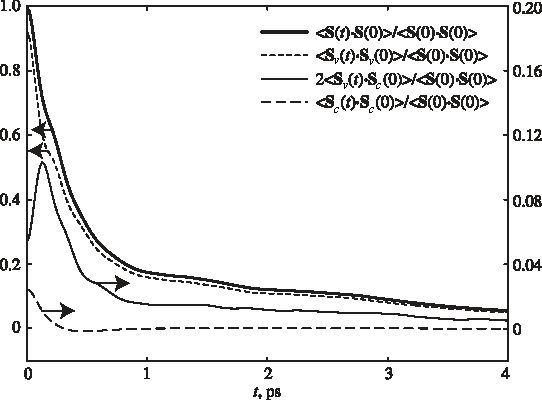
\includegraphics[width=8cm]{chapters/chapter2/figures/McGaughey-argon-contributions.pdf}
    \caption{Breakdown of the energy flux autocorrelation function $\langle\mathbf{J}^\smallE(t)\cdot\mathbf{J}^\smallE(t)\rangle$ of LJ fcc solid argon at $50\un{K}$ into the three terms of Eq.~\eqref{eq:JtJ0-components}. Note that the total ACF and the virial component correspond to the left vertical axis, while the cross and convection curves correspond to the right axis. Reproduced from Ref.~\cite{McGaughey2006}.}
    \label{fig:argon-convective}
\end{figure}

The first term on the right-hand side of Eq.~\eqref{eq:J-classical},
\begin{equation}
    \mathbf{J}_c = \frac{1}{\rOmega} \sum_n \mathbf{V}_n e_n , \label{eq:J-convective}
\end{equation}
is often called \emph{convective} (or \emph{kinetic}) and the second term,
\begin{equation}
    \mathbf{J}_v = \frac{1}{\rOmega} \left[ \sum_{n,m} (\mathbf{R}_n-\mathbf{R}_m) \mathbf{F}_{n m} \cdot \mathbf{V}_n \right], \label{eq:J-virial}
\end{equation}
is often called \emph{virial} (or \emph{potential}).
\citet{Fan2015} and \citet{Carbogno:2017gc}, for example, adopt this nomenclature and state that the convective term $\mathbf{J}_c$ ``\emph{gives no contributions to the conductivity tensor in solids, as mass transport is negligible}''.
We feel that the wording ``convective'' is somewhat misleading in this context, as the contribution of the convective current $\mathbf{J}_c$ to the heat conductivity may not vanish even in the absence of convection, especially in softer solid materials. 
Using Eqs.\eqref{eq:J-convective} and \eqref{eq:J-virial}, the energy flux autocorrelation function (ACF) can be split into 3 terms:
\begin{equation}
    \langle\mathbf{J}^\smallE(t)\cdot\mathbf{J}^\smallE(t)\rangle = \langle\mathbf{J}_c^\smallE(t)\cdot\mathbf{J}_c^\smallE(t)\rangle + 
    2\langle\mathbf{J}_c^\smallE(t)\cdot\mathbf{J}_v^\smallE(t)\rangle + 
    \langle\mathbf{J}_v^\smallE(t)\cdot\mathbf{J}_v^\smallE(t)\rangle . \label{eq:JtJ0-components}
\end{equation}
Their contributions to thermal conductivity were computed by \citet{McGaughey2006} for a LJ fcc argon crystal at $50\un{K}$ (the breakdown of $\langle\mathbf{J}^\smallE(t)\cdot\mathbf{J}^\smallE(t)\rangle$ into the three components in Eq.~\eqref{eq:JtJ0-components} is shown in Fig.~\ref{fig:argon-convective}). They found that while the convection contribution $\langle\mathbf{J}_c^\smallE(t)\cdot\mathbf{J}_c^\smallE(t)\rangle$ was indeed small ($\sim 1\%$), the contribution of the cross term $2\langle\mathbf{J}_c^\smallE(t)\cdot\mathbf{J}_v^\smallE(t)\rangle$ is not insignificant ($\sim 10\%$). The relative contribution of the convective and cross terms increase as the temperature goes up and anharmonic effects inhibit ``pure'' conduction. The absolute values of the convective contribution remains the same with increasing temperature, whereas the virial and cross term contributions decrease. While the convective term may not be as important for materials with higher thermal conductivity, in general, this contribution and (that of the cross term) should be checked before assuming they are negligible. Some further comments on this issue in Sec.~\ref{sec:carbogno}.

In the literature the nomenclature is often confusing, and this aspect not so well investigated. \citet{Vogelsang1987} divide the energy currents in two terms \cite{McQuarrie2000}: $\mathbf{J}^\smallE(\rGamma) = \mathbf{J}'_k + \mathbf{J}'_p$, where $\mathbf{J}'_k$ denotes the \emph{kinetic} part, defined as
\begin{equation}
    \mathbf{J}'_k = \frac{1}{\rOmega} \frac{(\mathbf{P}_n)^2}{2M_n} \mathbf{V}_n ,
\end{equation}
and $\mathbf{J}'_p$ denotes the \emph{potential} part, defined as
\begin{equation}
    \mathbf{J}'_p = \frac{1}{\rOmega} \left[ \sum_n  v_n(\{\mathbf{R}\}) \mathbf{V}_n + \sum_{n,m} (\mathbf{R}_n-\mathbf{R}_m) \mathbf{F}_{n m} \cdot \mathbf{V}_n \right] .
\end{equation}
They find that the kinetic term is negligible in solids, where atomic diffusion does not occour.

\citet{Kinaci2012}, instead, use the Einstein formulation and define a \emph{kinetic} term
\begin{equation}
    \mathbf{J}''_k = \frac{1}{\rOmega} \left[ \frac{(\mathbf{P}_n)^2}{2M_n} \mathbf{V}_n + \sum_{n,m} (\mathbf{R}_n-\mathbf{R}_m) \mathbf{F}_{n m} \cdot \mathbf{V}_n \right],
\end{equation}
and a \emph{potential} term
\begin{equation}
    \mathbf{J}''_p = \frac{1}{\rOmega} \sum_n  v_n(\{\mathbf{R}\}) \mathbf{V}_n ,
\end{equation}
and conclude that in perfect solid systems, where diffusion is highly improbable, $\mathbf{J}''_p$ contribution to thermal conductivity is negligible.

Finally, an alternative definition of the heat current can be used when dealing with solids \cite{Ladd1986}:
\begin{equation}
    \mathbf{J}^\smallE(\rGamma) =
       \frac{1}{\rOmega} \sum_{n,m} (\mathbf{R}_n^0 -\mathbf{R}_m^0) \mathbf{F}_{n m} \cdot \mathbf{V}_n , \label{eq:J-leyla}
\end{equation}
where $\mathbf{R}_n^0$ denotes the average atomic position of atom $n$. One should not confuse this expression with neglecting the convection part of the heat current. For a solid, Eq.~\eqref{eq:J-leyla} will give the same thermal conductivity as Eq.~\eqref{eq:J-classical-2body}, as demonstrated in Sec.~\ref{sec:carbogno}.


\paragraph{Many-body potentials}
In the case of a many-body potential interaction, if the atomic potential energy can be written as a function of the distance vectors $\mathbf{R_{nm}}=\mathbf{R}_n-\mathbf{R}_m$, as $v_n = v_n(\mathbf{R}_{1n},\mathbf{R}_{2n},\cdots,\mathbf{R}_{Nn})$, the force acting on atom $n$ can be written as \cite{Fan2015,Hardy2016}:
\begin{align}
    \mathbf{F}_n &= -\sum_m \frac{\partial v_m}{\partial \mathbf{R}_n} \\
        &= -\sum_{m\neq n} \frac{\partial v_m}{\partial \mathbf{R}_{nm}} + \sum_{p\neq n} \frac{\partial v_n}{\partial \mathbf{R}_{pn}} \\
        &= \sum_{m\neq n} \left(\frac{\partial v_m}{\partial \mathbf{R}_{nm}} + \sum_{p\neq n} \frac{\partial v_n}{\partial \mathbf{R}_{mn}} \right).
\end{align}
For example, for the Tersoff \cite{Tersoff1989} and Swillinger-Weber \cite{Stillinger1985} potentials, \citet{Fan2015} obtain the following definition for the virial energy flux:
\begin{equation}
    \mathbf{J}_v = \sum_n \sum_{n\neq m} \mathbf{R}_{ij} \left(\frac{\partial v_m}{\partial \mathbf{R}_{mn}} \cdot \mathbf{V}_n \right) ,
\end{equation}
equivalent to the one obtained by \citet{Hardy1963}, and they show that other two-body like formulations widely reported in the literature may give wrong results, especially in low-dimensional systems.

\end{LEtext}


\subsection{Multi-component fluids} \label{sec:multi-component}
In a multi-component fluid there is one conserved quantity (the particle number) per atomic species, plus the total energy and the three Cartesian components of the total momentum. The momentum densities are mass currents: the mass flux is therefore the total momentum, which vanishes in the center of mass reference frame. The transverse components of the momentum densities are decoupled from the other conserved densities \cite{Foster1975}, while the longitudinal one can be assumed to coincide with the total momentum in the long-wavelength limit. Momentum conservation thus constrains the number of fluxes interacting with the energy flux in Eq.~\eqref{eq:onsager} to $Q-1$, $Q$ being the number of atomic species, so that the resulting dimension of the matrix of Onsager coefficients, $L$, is $Q\times Q$. The heat flux is defined as the non-convective component of the energy flux, \emph{i.e.} the value of the latter in the absence of mass transport, that is to say when all the particle fluxes vanish.\footnote{It is unfortunate, but inevitable due to common usage, that this definition of non-convective flux clashes with a different definition given above while commenting Eq.~\eqref{eq:J-classical}.} By imposing this condition in Eq.~\eqref{eq:onsager}, with $\mathbf J^\smallone \equiv \mathbf{J}^\smallE$, and $\mathbf{J}^{q}$ ($q =2,\dots Q$) being independent particle fluxes, the thermal conductivity, defined as the ratio of the heat flux over the temperature gradient, is given by:
\begin{equation}
\kappa = \frac{1}{T^2 \,(L^{-1})^{\smallone\smallone}}. \label{eq:multi_kappa}
\end{equation}
This expression can be proved to be invariant under \textit{any} non-singular linear transformation of the independent particle fluxes. 

\paragraph{Two-component fluids}
For instance, in the case of a two-component liquid, energy and particle currents are coupled as in:
\begin{equation}
  \begin{aligned}
    \mathbf{J}^\smallE &= L^{\smallE\smallE}\,  \nabla \left (\frac{1}{T} \right ) + L^{\smallE\smallQ} \, \nabla \left (\frac{\mu}{T} \right ), \\
    \mathbf{J}^{\smallQ} &= L^{\smallE\smallQ} \, \nabla \left (\frac{1}{T} \right ) + L^{\smallQ\smallQ} \, \nabla \left (\frac{\mu}{T} \right ), \label{eq:two-comp-constitutive}
  \end{aligned}
\end{equation}
where $\mathbf{J}^{\smallQ}$ is the particle current of one of the two species (say, the second), and $\mu$ the corresponding chemical potential \cite{Sindzingre1990}. By imposing that the particle current vanishes, the resulting thermal conductivity is:
\begin{equation}
  \kappa=\frac{1}{T^2}
  \left( L^{\smallE\smallE} - \frac{(L^{\smallE\smallQ})^2}{L^{\smallQ\smallQ}} \right). \label{eq:two-comp-kappa}
\end{equation}


\bigskip
\bigskip
\LEnote{***** FINITE SIZE EFFECTS, QUANTUM EFFECTS ??? *****}